% =====================================================================
\chapter{Servicio a escala: latencia, rendimiento y memoria}
\label{tema:6}
% =====================================================================

Un servidor de inferencia recibe peticiones que llegan en momentos distintos, con prompts y respuestas de longitudes muy diferentes. Este tema define las métricas con las que se mide (tiempo hasta el primer token, tiempo por token y rendimiento), analiza por qué el \emph{batching} estático desperdicia el acelerador y cómo lo resuelve el \emph{batching} continuo, y estudia la gestión paginada de la caché KV, que elimina la fragmentación y permite compartir prefijos. Se siguen la clase~10 de CS336~\cite{cs336}, el artículo de Orca de Yu \emph{et al.}~\cite{orca}, las secciones~3 y~4 de Kwon \emph{et al.}~\cite{kwon} y la sección~2 de Pope \emph{et al.}~\cite{pope}.

\section{Métricas de servicio}

\begin{definicion}[Latencia y rendimiento]\label{def:metricas}
Para una petición, el \emph{tiempo hasta el primer token} ($\TTFT$) es el intervalo entre su llegada y la emisión del primer token de la respuesta; incluye la espera en cola y el \emph{prefill}. El \emph{tiempo por token de salida} ($\TPOT$) es el intervalo medio entre tokens sucesivos, y su inverso es la velocidad que percibe el usuario. El \emph{rendimiento} (\emph{throughput}) del sistema es el número total de tokens generados por segundo para todas las peticiones.
\end{definicion}

\begin{proposicion}[Latencia de una respuesta]\label{prop:latencia}
Una respuesta de $n_{\mathrm{out}}$ tokens se completa en $\TTFT+(n_{\mathrm{out}}-1)\,\TPOT$.
\end{proposicion}

\begin{proof}
El primer token llega en el instante $\TTFT$ y cada uno de los $n_{\mathrm{out}}-1$ restantes llega, en media, $\TPOT$ después del anterior.
\end{proof}

\begin{ejemplo}\label{ej:latencia}
Con $\TTFT=0{,}2$~s y $50$ tokens/s ($\TPOT=0{,}02$~s), una respuesta de $300$ tokens llega completa en $0{,}2+299\cdot 0{,}02=6{,}18$~s.
\end{ejemplo}

Las dos métricas dependen de fases distintas: el $\TTFT$ del \emph{prefill}, limitado por el cómputo, y el $\TPOT$ de la decodificación, limitada por la memoria (\cref{tema:2}). Por eso conviene procesar el \emph{prefill} con lotes pequeños, para reducir el $\TTFT$, y la decodificación con lotes grandes, para aumentar el rendimiento~\cite{cs336}. Además, replicar el modelo en $M$ grupos de aceleradores multiplica el rendimiento por $M$ sin cambiar la latencia, mientras que repartir un modelo entre aceleradores (módulo~17) reduce la latencia a cambio de comunicación~\cite{cs336,pope}.

\section{\emph{Batching} estático y continuo}

\begin{definicion}[\emph{Batching} estático]\label{def:estatico}
En el \emph{batching} estático, el servidor forma un lote de $B$ peticiones y lo ejecuta hasta que termina la más larga; solo entonces admite peticiones nuevas.
\end{definicion}

\begin{proposicion}[Utilización del lote estático]\label{prop:utilizacion}
Si las respuestas del lote tienen longitudes $\ell_1,\dots,\ell_B$, la fracción de ranuras de cómputo útiles durante la decodificación es
\[
U=\frac{\sum_{i=1}^{B}\ell_i}{B\,\max_i\ell_i}.
\]
\end{proposicion}

\begin{proof}
El lote ejecuta $\max_i\ell_i$ pasos con $B$ ranuras cada uno, en total $B\max_i\ell_i$ ranuras; de ellas, la petición $i$ ocupa $\ell_i$ y las demás quedan vacías o con relleno.
\end{proof}

\begin{definicion}[\emph{Batching} continuo]\label{def:continuo}
En el \emph{batching} continuo, o planificación por iteración, el servidor decide la composición del lote en cada paso de decodificación: cuando una secuencia termina, su ranura se asigna inmediatamente a una petición en espera~\cite{orca}. Como las secuencias tienen longitudes distintas, Orca aplica el \emph{batching selectivo}: las operaciones que actúan posición a posición (proyecciones y perceptrón) se ejecutan sobre la concatenación de todas las posiciones del lote, y la atención se calcula por separado para cada secuencia~\cite{orca,cs336}.
\end{definicion}

\begin{figure}[h]
\centering
\begin{tikzpicture}[font=\footnotesize,x=0.62cm,y=0.55cm]
  \node[font=\small] at (4,4.3) {estático};
  \node[font=\small] at (15,4.3) {continuo};
  \foreach \y/\l in {3/1,2/2,1/3} {\node[left] at (0,\y-0.5) {ranura \l}; \node[left] at (11,\y-0.5) {};}
  % estatico
  \draw[fill=black!15] (0,2.1) rectangle (3,2.9) node[midway] {$A$};
  \draw[pattern=north east lines,pattern color=regla] (3,2.1) rectangle (8,2.9);
  \draw[fill=black!30] (0,1.1) rectangle (8,1.9) node[midway] {$B$};
  \draw[fill=black!8] (0,0.1) rectangle (5,0.9) node[midway] {$C$};
  \draw[pattern=north east lines,pattern color=regla] (5,0.1) rectangle (8,0.9);
  \draw[->] (0,-0.2) -- (8.6,-0.2) node[right] {paso};
  % continuo
  \begin{scope}[xshift=6.82cm]
  \draw[fill=black!15] (0,2.1) rectangle (3,2.9) node[midway] {$A$};
  \draw[fill=black!45] (3,2.1) rectangle (8,2.9) node[midway,text=white] {$D$};
  \draw[fill=black!30] (0,1.1) rectangle (8,1.9) node[midway] {$B$};
  \draw[fill=black!8] (0,0.1) rectangle (5,0.9) node[midway] {$C$};
  \draw[fill=black!22] (5,0.1) rectangle (8,0.9) node[midway] {$E$};
  \draw[->] (0,-0.2) -- (8.6,-0.2) node[right] {paso};
  \end{scope}
\end{tikzpicture}
\caption{Tres ranuras durante ocho pasos de decodificación. Con \emph{batching} estático (izquierda), las ranuras de $A$ y $C$ quedan vacías (rayado) hasta que termina $B$: se usan 16 de 24 ranuras. Con \emph{batching} continuo (derecha), $D$ y $E$ entran en cuanto se liberan las ranuras y se usan las 24.}
\label{fig:batching}
\end{figure}

\begin{proposicion}[Utilización del \emph{batching} continuo]\label{prop:continuo}
Si en todo paso hay al menos tantas peticiones en espera como ranuras liberadas, el \emph{batching} continuo mantiene ocupadas todas las ranuras de decodificación.
\end{proposicion}

\begin{proof}
Al final de cada paso, cada ranura liberada recibe una petición en espera, que existe por hipótesis; ninguna ranura queda vacía en el paso siguiente.
\end{proof}

La proposición ignora el coste del \emph{prefill} de las peticiones que entran, que se intercala con la decodificación de las demás; su planificación es un problema propio de los sistemas de servicio.

\section{Memoria de la caché KV y PagedAttention}

Antes de vLLM, los servidores reservaban para cada petición un bloque contiguo de caché KV del tamaño máximo posible de la respuesta. Esa reserva produce \emph{fragmentación interna} (posiciones reservadas que nunca se usan) y \emph{fragmentación externa} (huecos entre reservas de tamaños distintos); en los sistemas que Kwon \emph{et al.} analizan, solo entre el $20{,}4\,\%$ y el $38{,}2\,\%$ de la memoria de la caché guarda estados de tokens~\cite[§1 y §3.1]{kwon}.

\begin{definicion}[PagedAttention]\label{def:paged}
\emph{PagedAttention} divide la caché KV de cada secuencia en \emph{bloques} de tamaño fijo de $b_{\mathrm{blk}}$ tokens, que no tienen por qué ser contiguos en memoria. Cada secuencia tiene una \emph{tabla de bloques} que traduce cada bloque lógico (posiciones $jb_{\mathrm{blk}},\dots,(j+1)b_{\mathrm{blk}}-1$) a un bloque físico. Los bloques se asignan cuando se llenan los anteriores, y el núcleo de atención lee la caché siguiendo la tabla~\cite[§4.1 y §4.2]{kwon}.
\end{definicion}

La analogía es la memoria virtual paginada de un sistema operativo: la secuencia ve un espacio lógico contiguo, formado por páginas físicas dispersas, y la tabla de bloques hace de tabla de páginas.

\begin{figure}[h]
\centering
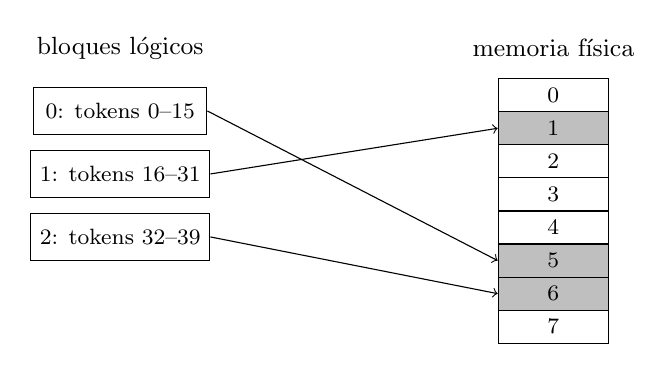
\begin{tikzpicture}[font=\footnotesize,
  lb/.style={draw,minimum width=2.2cm,minimum height=6mm},
  pb/.style={draw,minimum width=1.4cm,minimum height=4.2mm,inner sep=1pt}]
  \node[font=\small] at (0,1.0) {bloques lógicos};
  \node[lb] (l0) at (0,0.2) {0: tokens 0--15};
  \node[lb] (l1) at (0,-0.6) {1: tokens 16--31};
  \node[lb] (l2) at (0,-1.4) {2: tokens 32--39};
  \node[font=\small] at (5.5,1.0) {memoria física};
  \foreach \k in {0,...,7} \node[pb] (p\k) at (5.5,0.4-\k*0.42) {\k};
  \foreach \k in {1,5,6} \node[pb,fill=black!25] at (p\k) {\k};
  \draw[->] (l0.east) -- (p5.west);
  \draw[->] (l1.east) -- (p1.west);
  \draw[->] (l2.east) -- (p6.west);
\end{tikzpicture}
\caption{Una secuencia de 40 tokens con bloques de 16. La tabla de bloques ($0\mapsto 5$, $1\mapsto 1$, $2\mapsto 6$) la sitúa en tres bloques físicos no contiguos; solo se desperdician 8 posiciones del último bloque.}
\label{fig:paged}
\end{figure}

\begin{proposicion}[Desperdicio acotado]\label{prop:desperdicio}
Con bloques de $b_{\mathrm{blk}}$ tokens, una secuencia de $\ell\ge 1$ tokens ocupa $\lceil\ell/b_{\mathrm{blk}}\rceil$ bloques y desperdicia $b_{\mathrm{blk}}\lceil\ell/b_{\mathrm{blk}}\rceil-\ell\le b_{\mathrm{blk}}-1$ posiciones. Como todos los bloques tienen el mismo tamaño, no hay fragmentación externa: cualquier bloque libre sirve a cualquier secuencia.
\end{proposicion}

\begin{proof}
Por la definición de la parte entera superior, $b_{\mathrm{blk}}\lceil\ell/b_{\mathrm{blk}}\rceil$ es el menor múltiplo de $b_{\mathrm{blk}}$ mayor o igual que $\ell$, y su diferencia con $\ell$ es menor que $b_{\mathrm{blk}}$. Un bloque libre puede asignarse a cualquier entrada de cualquier tabla, porque la traducción no exige contigüidad.
\end{proof}

\begin{ejemplo}\label{ej:bloques}
Una respuesta de $300$ tokens con bloques de $16$ ocupa $\lceil 300/16\rceil=19$ bloques, $304$ posiciones, y desperdicia $4$. Con una reserva contigua de $2048$ posiciones desperdiciaría $1748$, el $85{,}4\,\%$. El tamaño de bloque por defecto de vLLM es $16$: bloques más pequeños desperdician menos, pero reducen el paralelismo de la lectura de la caché~\cite[§7.2]{kwon}.
\end{ejemplo}

\begin{proposicion}[Compartición de prefijos]\label{prop:prefijo}
Sean $n_s$ secuencias que comparten un prompt de $P$ tokens. Con compartición de bloques y \emph{copia en escritura}, el prompt ocupa $\lfloor P/b_{\mathrm{blk}}\rfloor$ bloques completos compartidos más, si $P$ no es múltiplo de $b_{\mathrm{blk}}$, una copia del bloque parcial por secuencia, en lugar de $n_s\lceil P/b_{\mathrm{blk}}\rceil$ bloques.
\end{proposicion}

\begin{proof}
Los bloques completos del prompt no se modifican nunca y pueden apuntarse desde las $n_s$ tablas, con un contador de referencias. El último bloque, si está incompleto, recibirá tokens distintos en cada secuencia; al primer intento de escritura se copia (copia en escritura), de modo que acaba habiendo una copia por secuencia~\cite[§4.3 y §4.4]{kwon}.
\end{proof}

Este mecanismo sirve para el muestreo de varias respuestas por prompt, para la búsqueda en haz y para los prompts de sistema comunes. Las API públicas de Anthropic y de Google ofrecen una caché de prefijos del prompt (\emph{prompt caching} y \emph{context caching}) como función documentada; su implementación interna no es pública.

\begin{lecturas}
\item CS336~\cite{cs336}, clase~10 «Inference»: \emph{throughput and latency}, \emph{continuous batching} y \emph{paged attention}.
\item Yu \emph{et al.}~\cite{orca}, planificación por iteración y \emph{batching} selectivo.
\item Kwon \emph{et al.}~\cite{kwon}, secciones~3 («Memory Challenges in LLM Serving») y~4 («Method»), y §7.2.
\item Pope \emph{et al.}~\cite{pope}, sección~2 «Inference Cost Tradeoffs».
\end{lecturas}

\section*{Ejercicios del tema 6}
\addcontentsline{toc}{section}{Ejercicios del tema 6}

\begin{ejercicio}{1}{eje:6-paginacion}
Explique con la analogía de la memoria virtual de un sistema operativo qué problemas resuelve PagedAttention y qué papel tiene la tabla de bloques. ¿Qué equivale a compartir una página de solo lectura entre procesos?
\end{ejercicio}

\begin{ejercicio}{2}{eje:6-bloques}
Una petición con $1000$ tokens de caché se guarda en bloques de $16$. ¿Cuántos bloques ocupa y cuántas posiciones desperdicia? Compárelo con una reserva contigua de $2048$ posiciones.
\end{ejercicio}

\begin{ejercicio}{2}{eje:6-latencia}
(a) Un modelo de $1{,}3\cdot 10^{10}$ parámetros en fp16 se sirve con lote~1 en un acelerador de $300$~TFLOP/s, aprovechado al $50\,\%$ en el \emph{prefill}, y $1$~TB/s. Para un prompt de $2000$ tokens y una respuesta de $500$, estime el $\TTFT$ (sin cola), el $\TPOT$ y la latencia total. (b) Un lote estático de 4 peticiones tiene respuestas de $100$, $400$, $250$ y $50$ tokens. Calcule su utilización.
\end{ejercicio}

\begin{ejercicio}{2}{eje:6-gqa}
Continúe el \cref{eje:2-llama13}. Con GQA de $8$ cabezas de clave y valor, los parámetros bajan a $1{,}1338\cdot 10^{10}$ (las proyecciones de clave y valor se reducen). Con los mismos supuestos, calcule la caché por secuencia y, para $B=64$ y $B=256$, la memoria total, la latencia y el rendimiento. ¿Caben en 80~GB? Compare con la atención multicabeza.
\fuente{adaptado de CS336~\cite{cs336}, clase~10 «Inference», apartado \emph{reduce KV cache size} (GQA en Llama~2 13B).}
\end{ejercicio}

\begin{ejercicio}{2}{eje:6-prefijo}
Cuatro muestras de una misma petición comparten un prompt de $1000$ tokens, con bloques de $16$ y la caché de Llama~2 7B ($512$~KiB por token). Calcule los bloques del prompt sin y con compartición y la memoria ahorrada.
\end{ejercicio}

\begin{ejercicio}{3}{eje:6-frag}
(a) Suponga que la longitud $\ell$ de las secuencias es tal que $\ell\bmod b_{\mathrm{blk}}$ es uniforme en $\{0,\dots,b_{\mathrm{blk}}-1\}$. Demuestre que el desperdicio esperado por secuencia con PagedAttention es $(b_{\mathrm{blk}}-1)/2$. (b) Si las longitudes son uniformes en $\{1,\dots,L_{\max}\}$ y se reservan $L_{\max}$ posiciones contiguas, demuestre que el desperdicio esperado es $(L_{\max}-1)/2$. (c) Calcule ambos para $b_{\mathrm{blk}}=16$ y $L_{\max}=2048$.
\end{ejercicio}
